%% Nature Communications Article, Springer Nature LaTeX template v3.1 (December 2024), sn-nature style.
%% Draft v4.1 (6 October 2026; author edits of 6 Oct merged, figures redesigned). Draft v4 (6 October 2026): method = residual-calibrated hedging (RCH), option A after the method studies; v3 in ../archive/main_v3_before_rch.tex (option B after the
%% novelty audit, ../NOVELTY_AUDIT.md). v2 is in ../archive/main_v2_committed_prefix.tex.
%% All experiments are reported. Remaining \pending{...} items are author details (DOIs, funding, CRediT).
%% Pilot numbers come from one model per family and task and are labelled as such.

\documentclass[pdflatex,sn-nature]{sn-jnl}

\usepackage{graphicx}
\usepackage{multirow}
\usepackage{amsmath,amssymb,amsfonts}
\usepackage{amsthm}
\usepackage{xcolor}
\usepackage{booktabs}
\usepackage{algorithm}
\usepackage{algorithmicx}
\usepackage{algpseudocode}
\usepackage{url}

\theoremstyle{thmstylethree}
\newtheorem{definition}{Definition}

\newcommand{\pending}[1]{\textcolor{red}{[PENDING: #1]}}
\newcommand{\ceil}[1]{\left\lceil #1 \right\rceil}

\raggedbottom

\begin{document}

\title[Hedging prediction error through inference delay]{Hedging against prediction error through inference delay in world-model planning}

\author[1]{\fnm{Runze} \sur{Xia}}
\author*[1]{\fnm{Richard} \sur{Jiang}}\email{r.jiang2@lancaster.ac.uk}
\affil*[1]{\orgdiv{School of Computing and Communications}, \orgname{Lancaster University}, \orgaddress{\city{Lancaster}, \country{UK}}}
%% Confirm the department and author details before submission.

\abstract{World-model planners take time to compute while a deployed system keeps moving. Predicting the state at which a plan takes effect is the standard remedy, but with learned world models it leaves most of the delay loss, because their errors through the delay are value-aligned. We propose residual-calibrated hedging, a training-free addition to sampling-based planners that scores each candidate over post-delay states formed from the world model's prediction and its own recorded errors. Scored in one batched call, four such states add no measurable latency for one robot. In pre-registered tests on 24 recurrent, joint-embedding and TD-MPC2 world models, hedging over four states improved on predictive compensation at delays of four and eight decisions; sixteen states improved it only at eight. In secondary comparisons, the four-state gain held on held-out models and doubled predictive compensation's gain over time-aligned execution. Ablations show that point corrections and predictability penalties do not help.}

\keywords{world models, model predictive control, inference latency, delay compensation, robust planning}

\maketitle

%% ------------------------------------------------------------------ Introduction
\section{Introduction}\label{sec:intro}

Learned world models let an agent evaluate actions before taking them\cite{ha2018world,finn2017foresight}. In model predictive control\cite{mayne2000constrained,rawlings2017mpc}, a sampling-based planner proposes candidate action sequences, the model predicts their consequences, and the best sequence is executed, with planning repeated as observations arrive. The planner is typically model predictive path integral control (MPPI)\cite{williams2016aggressive,williams2017mppi} or the cross-entropy method\cite{rubinstein1999cem,pinneri2020icem}, and this loop has been used with learned models from pixels\cite{hafner2019planet,chua2018pets,hansen2022tdmpc,hansen2023tdmpc2}. Learned models also drive tree search\cite{schrittwieser2020muzero} and policy learning in imagination\cite{hafner2020dreamer,hafner2023dreamerv3}.

The models range widely in size:
\begin{itemize}
\item compact recurrent state-space models\cite{hafner2019planet};
\item joint-embedding predictors\cite{maes2026lewm,zhou2024dinowm};
\item video world models with hundreds of millions to billions of parameters\cite{zhao2026miniworld,wu2024ivideogpt,alonso2024diamond,nvidia2025cosmos}.
\end{itemize}
Their planning calls take from milliseconds to minutes.

While a planner computes, a physical system keeps moving and executes actions that were committed earlier. Delayed decision processes have long been studied\cite{katsikopoulos2003delays}. Reinforcement learning has formalised the real-time setting\cite{ramstedt2019rtrl,xiao2020thinking,ramstedt2020random,riemer2024staggered} and benchmarked algorithms in it\cite{thodoroff2022benchmarking}. Control theory has a standard remedy: predict, with the model, the state at which the new control will be applied, and optimise from there\cite{smith1957dead,findeisen2004computational,dirckx2024asap}. The same remedy appears in several other settings:
\begin{itemize}
\item delay-aware model-based reinforcement learning\cite{chen2020dats,karamzade2025random};
\item model predictive control with learned models on robots\cite{elasri2025rthcp};
\item tree search that simulates the committed steps\cite{muppidi2026time};
\item action-chunking policies\cite{zhao2023act,chi2023diffusionpolicy}, as conditioning on the pending actions or on forecasts of the state at execution time\cite{black2025rtc,shukor2025smolvla,wang2026rapac,motubrain2026wamrt,liao2025dadp,jiang2026futurertc,ye2026dreamzero}.
\end{itemize} We call it committed-prefix planning. With an exact model it loses nothing except replanning frequency\cite{findeisen2004computational}.

Learned world models are not exact. Their multi-step predictions drift\cite{janner2019mbpo}, and their training objective is not the planner's\cite{lambert2020objective}. How much of the delay loss committed-prefix planning recovers with such models has not been measured. We measure it for three families of pixel world models on three control tasks, splitting the delay loss into a feedback-rate term and a prediction-mismatch term in the manner of networked predictive control\cite{beger2025optimal}. Committed-prefix planning removes only about 30\% of the mismatch. The remaining loss is not explained by the size of the prediction error: on the same states, a random error of the same size costs one-third to three-quarters as much as the model's actual error, so the actual errors fall along directions that matter for the plan's value. Corrections that assume small or low-dimensional errors do not help: neither a first-order sensitivity update\cite{zavala2009asnmpc,belvedere2026feedback} nor bias removal.

We therefore propose residual-calibrated hedging (RCH), a training-free addition to any sampling-based planner that uses a learned world model.

\textbf{Calibration.} Before deployment, the model's own errors in predicting through committed actions are recorded on its training data.

\textbf{Planning.} At each call, every candidate action sequence is scored by its average predicted cost over several post-delay states: the model's prediction, plus errors drawn from that record. A learned variant replaces the record with a small heteroscedastic error model conditioned on the state and the committed actions.

The idea of hedging over the execution-time state comes from robust and scenario-based predictive control\cite{calafiore2006scenario,lucia2013multistage,dyro2021particle,gandhi2021robust}. CLIS-MPPI\cite{liu2026clis} applied it to planning delay in MPPI: it optimises rollouts from sampled execution-time initial states and corrects the executed actions with rollout-based feedback, using a known robot model. RCH makes this kind of hedging work for learned world models, whose dominant uncertainty is model error rather than the length of the delay. The hedge distribution is calibrated from the model's own measured errors, not from an assumed delay distribution or an ensemble of probabilistic models\cite{chua2018pets,chen2020dats}. RCH therefore applies to any single pretrained world model, including deterministic latent models and video diffusion models. It also costs almost no latency: a single robot's planning call is limited by the sequential steps of the model rollout rather than by the number of candidate rows, so the hedge states can be scored in the same batched call.

Our contributions are:
\begin{itemize}
\item \textbf{The method.} Residual-calibrated hedging, an algorithm and a deployment recipe for sampling-based planners with learned world models, with a learned heteroscedastic variant (Algorithm~\ref{alg:hedge}, Section~\ref{sec:method}).
\item \textbf{Why it is needed.} With learned pixel world models, committed-prefix planning leaves about 70\% of the mismatch loss, because the models' errors through the delay are value-aligned (Fig.~\ref{fig:curves}, Table~\ref{tab:diag}).
\item \textbf{Evidence.} Pre-registered tests on 24 world models in three families: four anchors improve on committed-prefix planning at delays of four and eight decisions, and sixteen anchors only at eight. A second study on held-out models and its ablations, where these gains are secondary comparisons, shows that the gain comes from hedging rather than from correcting the prediction or penalising uncertainty (Tables~\ref{tab:contrasts} and~\ref{tab:heldout}). Batched scoring keeps it at the latency of plain planning (Table~\ref{tab:latency}).
\end{itemize}

%% ------------------------------------------------------------------ Results
\section{Results}\label{sec:results}

\subsection{Paused simulators hide the latency of world-model planners}\label{sec:motivation}

Closed-loop evaluations of world-model planners almost always pause the simulator during planning\cite{tassa2018dmc,maes2026swm,zhang2025worldinworld}. Timing records from a configuration study of a diffusion world-model planner show what this can hide (Fig.~\ref{fig:motivation}). The planner is a MiniWorld-0.5B video model\cite{zhao2026miniworld} fine-tuned on DeepMind Control Suite data and planned with model predictive path integral control (MPPI)\cite{williams2017mppi}. Across six inference configurations, the amortised planning cost fell 3.41-fold, from 10.44 to 3.06 seconds per decision. The duration of one planning call fell only from 209 to 121 seconds, longer than the 10 to 25 seconds of simulated time in a whole episode. Planning less often halved the amortised cost and left the call duration unchanged. Throughput and latency are distinct measures of inference cost\cite{reddi2019mlperf}, and only latency determines how stale a plan is. Fewer sampler steps\cite{song2021ddim} shortened the call, but nowhere near a control period. Timed for a single environment on the same GPU, one call with two sampler steps took 28 s, about 1,400 cartpole decisions. Throughout this paper, latency means the duration of one planning call, and the delay $d$ is the number of decisions that elapse during it.

\begin{figure}[t]
\centering
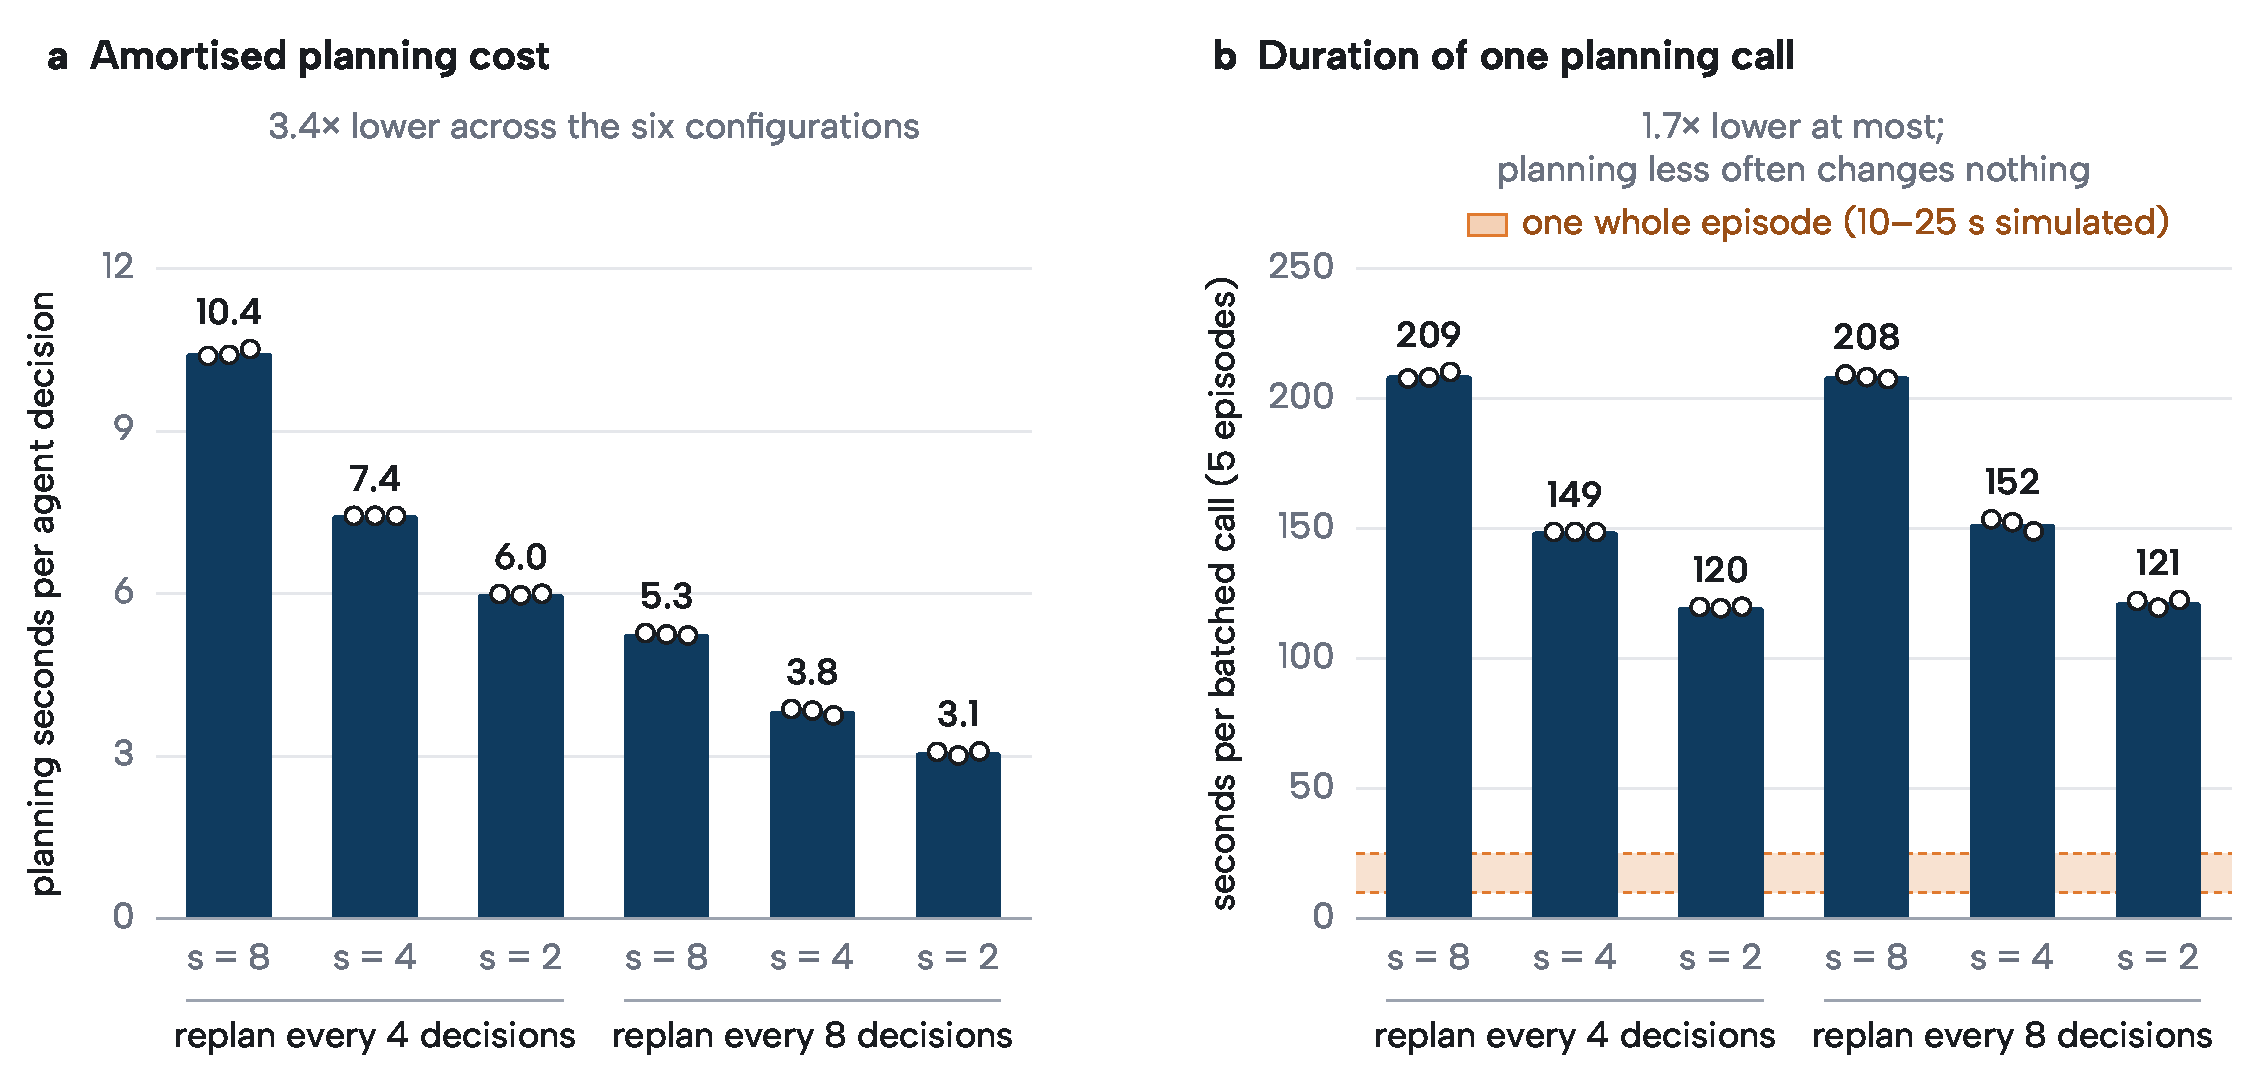
\includegraphics[width=\textwidth]{../figures/cost_vs_latency.pdf}
\caption{\textbf{Amortised planning cost and the duration of a planning call measure different things.} Reanalysis of an 18-job configuration study of a diffusion world-model planner on one V100 GPU (three DeepMind Control tasks, five episodes per task and configuration, simulator paused while planning). Bars are grouped by the number of decisions $r$ served by one planning call, and $s$ is the number of sampler steps. \textbf{a}, Planning seconds per agent decision, averaged over tasks. \textbf{b}, Mean duration of one planning call serving five batched episodes, reconstructed from accumulated timers and the number of calls (Methods). The shaded band marks the simulated duration of a whole episode (10--25 s). No timing intervals are shown because independent timing repetitions were not recorded.}
\label{fig:motivation}
\end{figure}

\subsection{Committed-prefix planning leaves a residual mismatch}\label{sec:residual}

We ran recurrent state-space (RSSM)\cite{hafner2019planet}, joint-embedding predictive (JEPA)\cite{maes2026lewm} and TD-MPC2\cite{hansen2023tdmpc2} world models on cartpole swing-up, walker walk and cup catch\cite{tassa2018dmc}, with three independently trained models per family and task. Each model was evaluated under delays of $d\in\{1,2,4,8,16\}$ decisions, with 50 episodes per condition starting from states shared across conditions (Methods). Four schedules were compared (Fig.~\ref{fig:schematic}):
\begin{itemize}
\item the paused planner $\mathcal{P}_r$, where the simulator waits during planning and $r$ actions are executed per plan;
\item the naive planner $\mathcal{N}_d$, which executes a plan made for an earlier state from its first action;
\item the time-aligned planner $\mathcal{A}_d$, which executes the same plan from position $d$;
\item committed-prefix planning $\mathcal{C}_d$.
\end{itemize}
The asynchronous planners make identical model calls. With an exact model, $\mathcal{C}_d$ reproduces $\mathcal{P}_d$, so its loss relative to $\mathcal{P}_d$ measures prediction mismatch alone (Methods).

\begin{figure}[t]
\centering
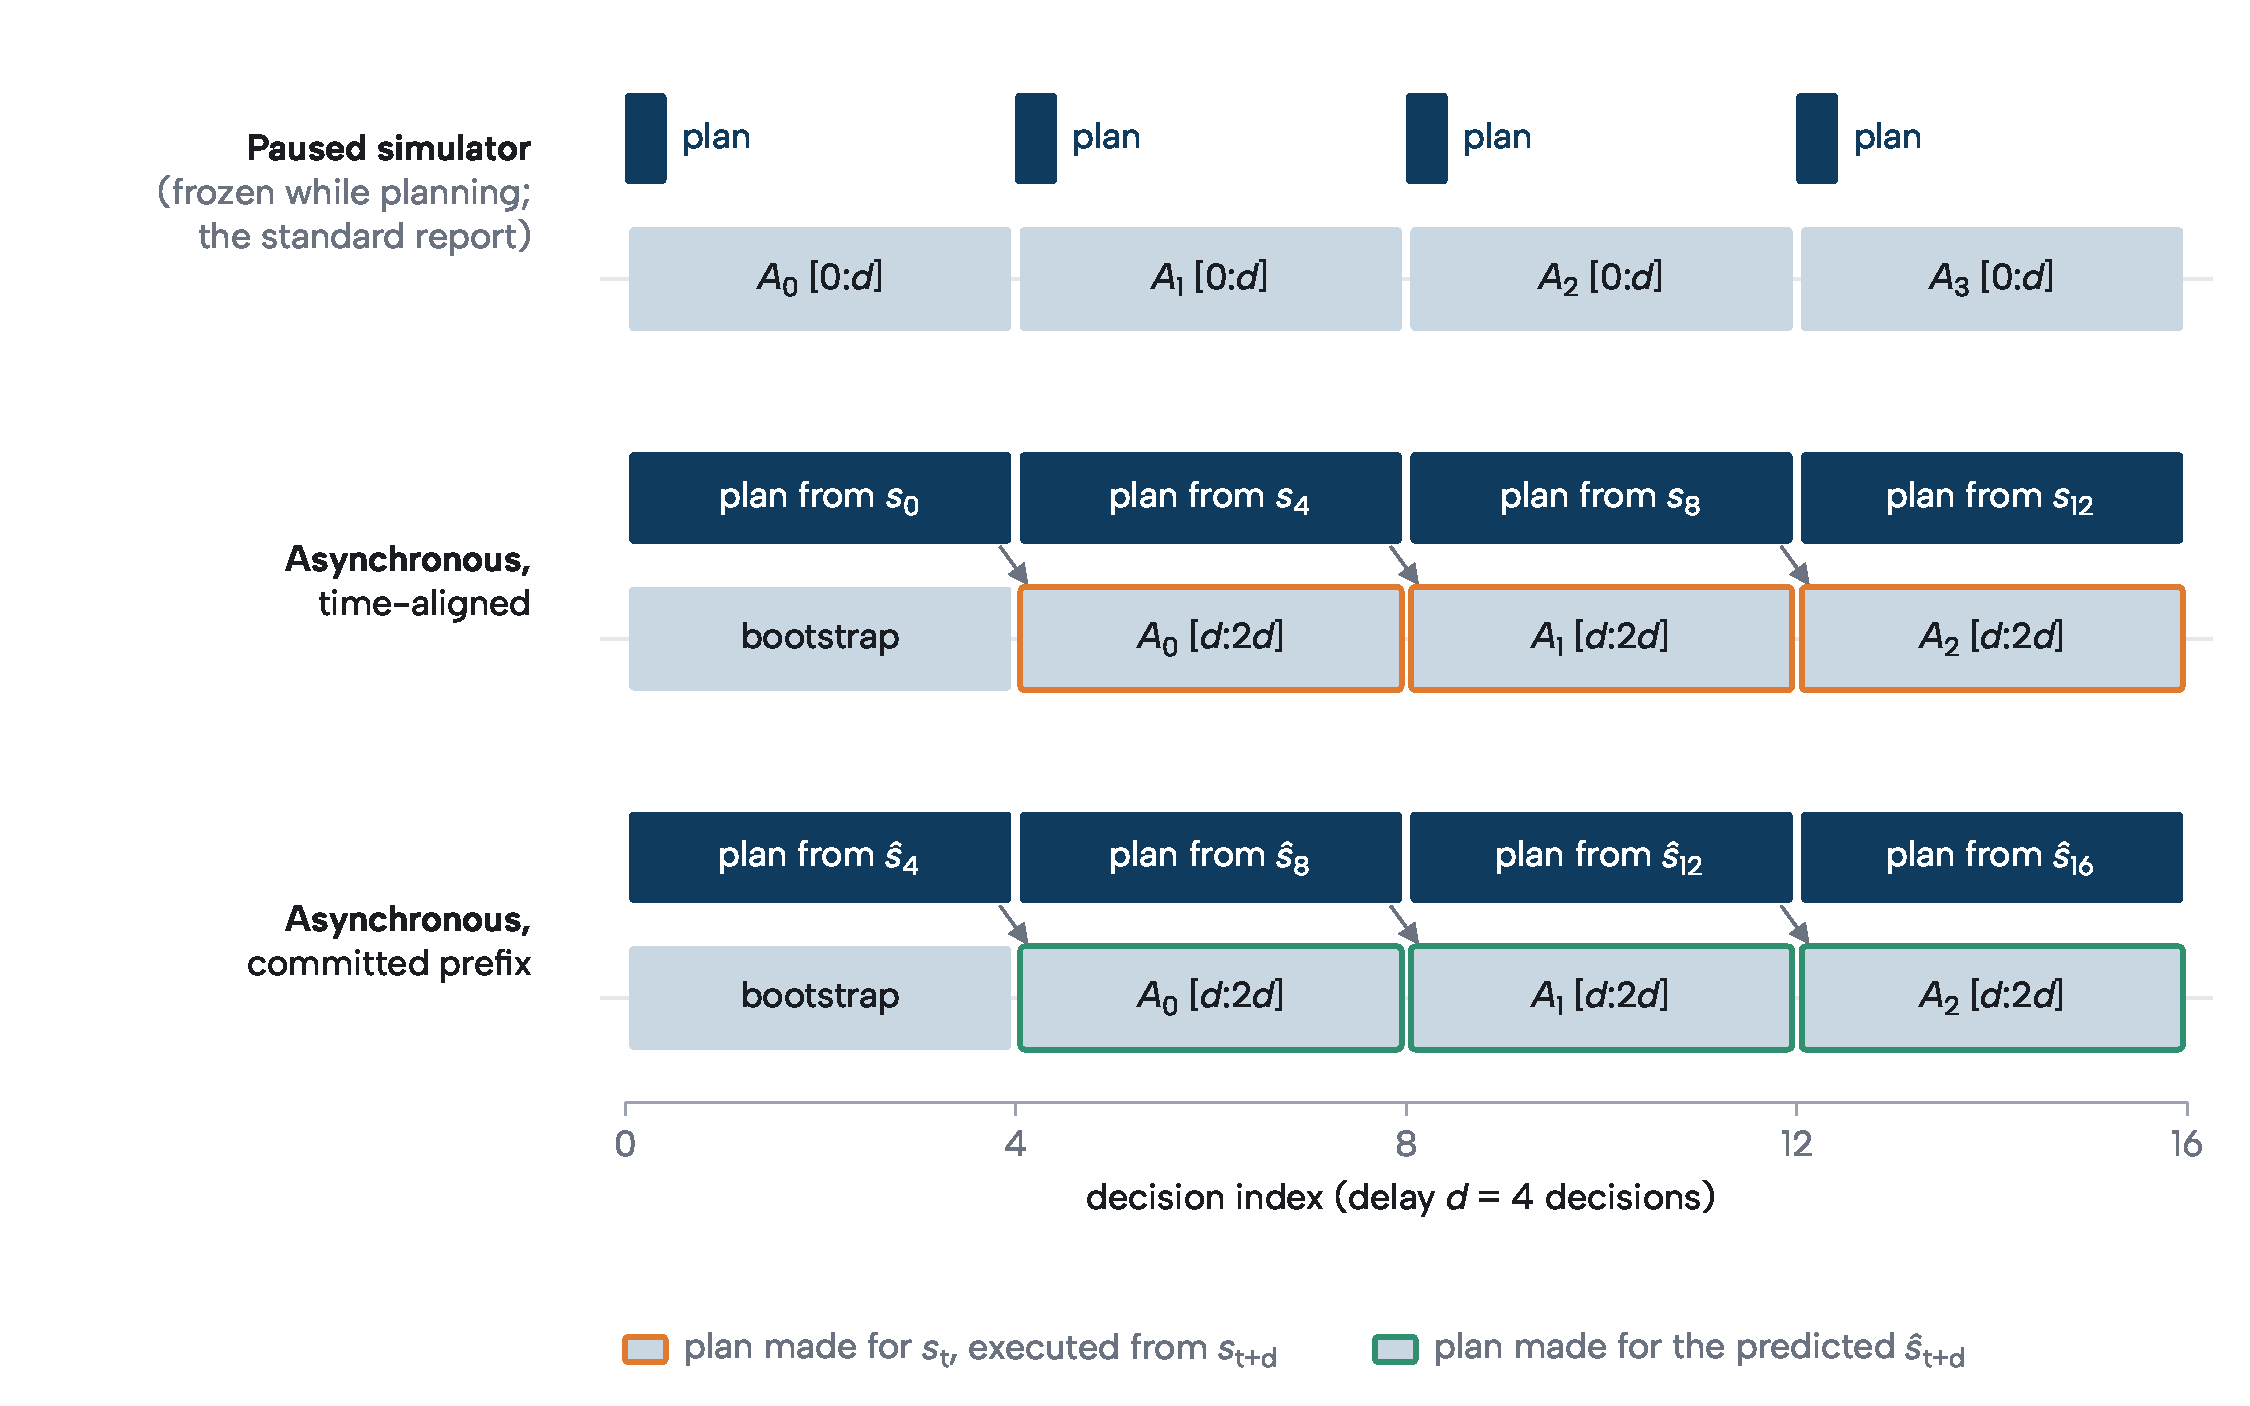
\includegraphics[width=\textwidth]{../figures/cpp_timeline.pdf}
\caption{\textbf{Planning schedules under a delay of $d=4$ decisions.} Top, the paused reference, in which the simulator is frozen during each plan. Middle, time-aligned asynchronous planning: each call plans from the observation at its start and its actions from position $d$ onward are executed after the call returns, from a state the plan did not assume (orange outline). Bottom, committed-prefix planning: each call rolls the world model through the actions that will execute during the call and plans from the predicted state $\hat s_{t+d}$ (green outline). Residual-calibrated hedging keeps this schedule and changes how candidates are scored (Algorithm~\ref{alg:hedge}).}
\label{fig:schematic}
\end{figure}

Committed-prefix planning beat time-aligned planning at every delay, and the margin grew with the delay. Pooled over the eight family--task cells above the pre-specified return floor, the margin rose from $+0.010$ normalised return at $d=1$ to $+0.048$ $[+0.028, +0.068]$ at $d=16$ (Fig.~\ref{fig:curves}a). The pre-registered test that the margin is positive at each of $d=2,4,8$ just failed, with $p=0.050$. The naive planner was far worse than either.

Splitting the delay loss shows where the return goes (Fig.~\ref{fig:curves}b). Up to $d=8$, most of it is mismatch rather than reduced feedback. At $d=8$, the time-aligned planner loses $0.133$ $[0.104, 0.163]$ to mismatch and $0.080$ $[0.047, 0.115]$ to replanning less often. Committed-prefix planning reduces the mismatch to $0.092$ $[0.072, 0.114]$, which removes 31\% of it. Across delays it removes 27--36\%, against the pre-registered expectation of at least half.

\begin{figure}[t]
\centering
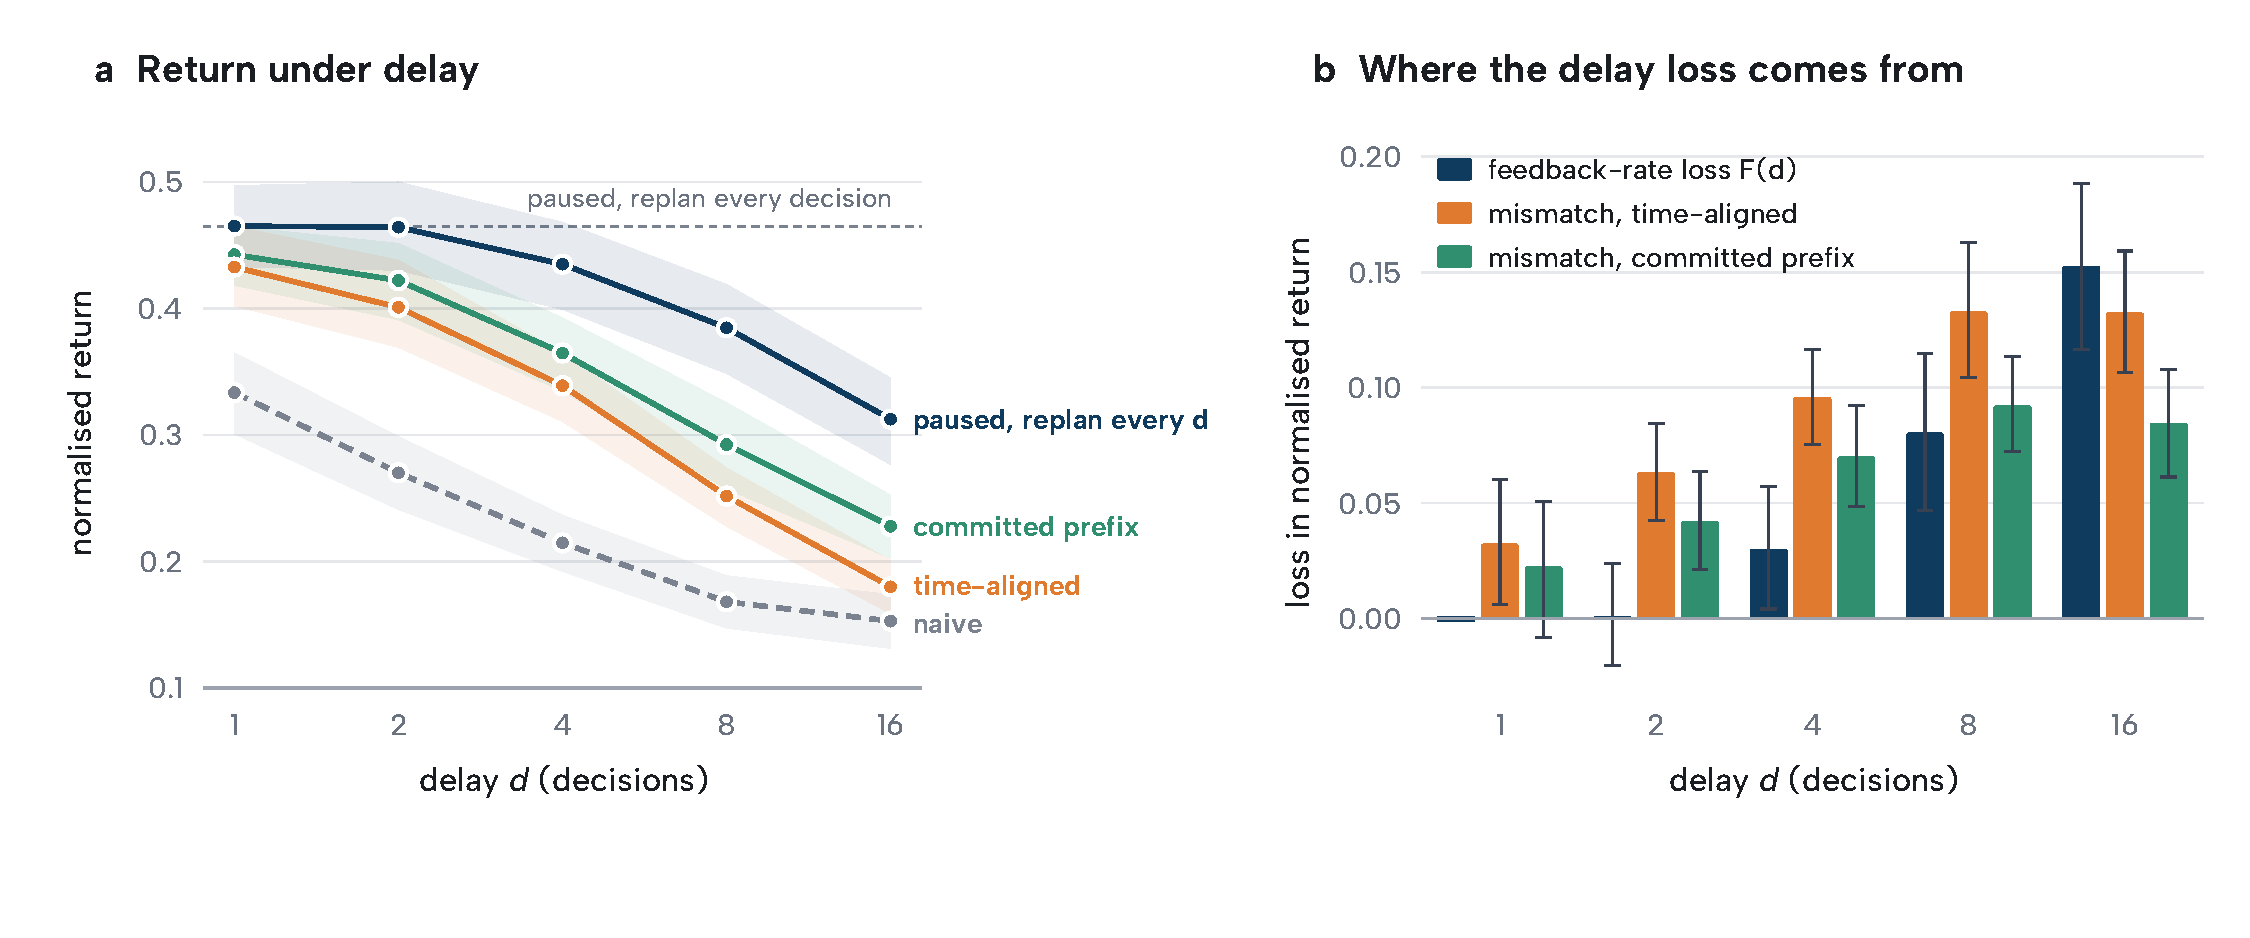
\includegraphics[width=\textwidth]{../figures/delay_curves.pdf}
\caption{\textbf{Committed-prefix planning recovers a minority of the delay loss with learned world models.} RSSM, JEPA and TD-MPC2 world models on three DeepMind Control tasks, eight family--task cells above the return floor, three models per cell, 50 episodes per model and condition. \textbf{a}, Normalised return against delay for each schedule; the dashed line marks the paused planner that replans every decision. Bands are 95\% hierarchical bootstrap intervals of each schedule's pooled mean; paired contrasts between schedules are tighter (main text). \textbf{b}, Delay loss of the asynchronous planners split into feedback-rate loss $F(d)=R(\mathcal{P}_1)-R(\mathcal{P}_d)$ and mismatch loss $M(d)=R(\mathcal{P}_d)-R(\mathcal{X}_d)$, with 95\% intervals.}
\label{fig:curves}
\end{figure}

\subsection{The residual comes from value-aligned prediction errors}\label{sec:diagnosis}

To find what limits committed-prefix planning, we replayed held-out data windows with each model, used the recorded actions as the committed prefix, and planned once from the predicted post-delay latent and once from the true filtered latent, with identical sampling noise (Methods). Regret is the model-predicted cost of the plan from the predicted latent, evaluated from the true latent, minus that of the plan made from the true latent. Replanning from the true latent with different noise gives regret near zero, so the regret reflects the anchor rather than sampling variance.

The predicted latent was close to the truth: its error was under 20\% of the stale error for the RSSM and JEPA models, and 7--140\% for TD-MPC2. Regret was nonetheless large wherever committed-prefix planning had failed in closed loop (Table~\ref{tab:diag}). Replacing the model's error by a random error of the same size reduced regret by a factor of 1.3 to 3, so the actual errors fall along value-relevant directions. Halving the error roughly halved the regret. Two corrections failed:
\begin{itemize}
\item a finite-difference sensitivity correction along the eight leading directions of calibration residuals, which held only 10--50\% of the error;
\item removing the mean residual.
\end{itemize}
Selecting, on arrival, the plan of whichever of 16 candidate anchors lay nearest the observed state also barely helped. Scoring each candidate by its average cost over anchors drawn from calibration residuals reduced regret by roughly a quarter to a half wherever there was regret to remove (more in one noisy case).

\begin{table}[t]
\caption{\textbf{Anchor regret on held-out windows at $d=2$.} Model-predicted cost from the true post-delay latent of the plan made from each anchor, minus that of the plan made from the true latent (model cost units, 64 windows). Hedged: one plan scored by the mean cost over 16 anchors, the predicted latent plus 15 calibration residuals. RSSM cup is a control where committed-prefix planning already works.}\label{tab:diag}
\begin{tabular*}{\textwidth}{@{\extracolsep\fill}lrrrrr@{}}
\toprule
Model
& \multicolumn{1}{c}{\shortstack{Stale\\latent}}
& \multicolumn{1}{c}{\shortstack{Predicted\\latent}}
& \multicolumn{1}{c}{\shortstack{Random error,\\same size}}
& \multicolumn{1}{c}{\shortstack{Half the\\error}}
& \multicolumn{1}{c}{\shortstack{Hedged,\\$K=16$}} \\
\midrule
RSSM walker & 16.28 & 7.84 & 3.90 & 3.94 & 3.59 \\
JEPA cartpole & 0.58 & 0.45 & 0.14 & 0.18 & 0.32 \\
TD-MPC2 walker & 6.08 & 3.65 & 2.72 & 2.94 & 2.77 \\
TD-MPC2 cup & 2.68 & 1.65 & 0.82 & 0.42 & $-1.55$ \\
RSSM cup & 2.95 & $-0.02$ & 0.00 & $-0.03$ & $-0.03$ \\
\botrule
\end{tabular*}
\end{table}

\subsection{Residual-calibrated hedging}\label{sec:method}

Residual-calibrated hedging keeps the committed-prefix schedule and changes only how a candidate is scored (Algorithm~\ref{alg:hedge}).

\textbf{Calibration, once per model and delay.} The model's own $d$-step prediction residuals $r = z_{t+d} - \hat z_{t+d}$ are recorded on training windows, giving a bank of 512 residuals. The learned variant instead fits a small network to the same residuals, conditioned on $\hat z_{t+d}$, $z_t$ and the committed actions; it predicts the residual's mean and per-dimension variance (Methods).

\textbf{At each call.}
\begin{itemize}
\item The committed actions are rolled through the model once, giving the predicted latent $\hat z$.
\item $K$ anchors are formed: $\hat z$ itself, and $\hat z$ plus $K-1$ residuals drawn from the bank. In the learned variant, the anchors are the corrected mean and $K-1$ draws from the predicted distribution.
\item Each candidate's free actions are scored by the mean predicted cost over the anchors, using the same samples for every anchor, in one batched call.
\end{itemize}

With $K=1$ the method is committed-prefix planning. The hedge targets the failure diagnosed above: a plan tuned to one predicted state is fragile when the error falls in value-relevant directions, and averaging over plausible post-delay states favours plans that are good across them.

\textbf{Deployment recipe.}
\begin{enumerate}
\item Measure the latency of the whole control loop, including frame encoding, and set $d$ to its 95th percentile divided by the decision period, rounded up (Section~\ref{sec:wallclock}).
\item Record the residual bank for that $d$ from the model's training data. This takes minutes and needs no retraining.
\item Hedge over $K=4$ anchors at the planner's usual population, scoring them in one batch. Do not reduce the population to make room for anchors (Table~\ref{tab:contrasts}).
\end{enumerate}

\subsection{Four-anchor hedging recovers return at delays of four decisions or more}\label{sec:closedloop}

Over all 24 models, the pre-registered test of 16 anchors against committed-prefix planning confirmed a gain at $d=8$ but not at $d=4$ (Table~\ref{tab:contrasts}):
\begin{itemize}
\item $d=8$: $+0.036$ $[+0.014, +0.057]$ normalised return, Holm-adjusted one-sided $p=0.0014$;
\item $d=4$: $+0.008$ $[-0.010, +0.027]$, $p=0.19$, so the pilot's marginal gain did not replicate.
\end{itemize}
The pre-registered equal-latency test of four anchors, which add no latency for a single environment (Section~\ref{sec:latency}), succeeded at both delays: $+0.022$ $[+0.003, +0.040]$ at $d=4$ (Holm-adjusted one-sided $p=0.035$) and $+0.037$ $[+0.016, +0.058]$ at $d=8$ ($p=0.0004$). Neither number of anchors helped at $d=2$, where little mismatch remains.

Against time-aligned planning, the common asynchronous baseline, four-anchor hedging doubled the gain of committed-prefix planning (secondary contrasts):

\begin{center}
\begin{tabular}{@{}lrr@{}}
\toprule
 & \multicolumn{1}{c}{$d=4$} & \multicolumn{1}{c}{$d=8$} \\
\midrule
Committed prefix vs time-aligned & $+0.020$ & $+0.035$ \\
Hedged ($K=4$) vs time-aligned & \shortstack[r]{$+0.042$\\$[+0.024, +0.060]$} & \shortstack[r]{$+0.072$\\$[+0.047, +0.098]$} \\
\botrule
\end{tabular}
\end{center}

In the single-model pilot, gains were largest where diagnosis had found value-aligned errors, for example JEPA cup catch at $d=8$ (0.43 to 0.68 with 16 anchors) and RSSM walker (0.13 to 0.17). Hedging hurt slightly on JEPA cartpole and on TD-MPC2 cartpole and walker.

\begin{table}[t]
\caption{\textbf{Closed-loop contrasts over 24 models.} Difference in normalised return, pooled with equal weight over eight family--task cells (three models each, 50 episodes per model and arm, shared initial states). 95\% hierarchical bootstrap intervals; one-sided $p$, Holm-adjusted within each pre-specified family (Supplementary Note~1). $K$: anchors; $N$: population. All arms use 6 MPPI iterations and horizon 32.}\label{tab:contrasts}
\begin{tabular*}{\textwidth}{@{\extracolsep\fill}llccc}
\toprule
Family & Contrast & $d$ & Difference [95\% CI] & $p$ (Holm) \\
\midrule
Replication & $K=16$ vs $K=1$, $N=512$ & 4 & $+0.008$ $[-0.010, +0.027]$ & 0.19 \\
 & & 8 & $+0.036$ $[+0.014, +0.057]$ & 0.0014 \\
Equal latency & $K=4$, $N=512$ vs $K=1$, $N=512$ & 4 & $+0.022$ $[+0.003, +0.040]$ & 0.035 \\
 & & 8 & $+0.037$ $[+0.016, +0.058]$ & 0.0004 \\
 & $K=16$, $N=128$ vs $K=1$, $N=512$ & 4 & $-0.034$ $[-0.053, -0.015]$ & 1.0 \\
 & & 8 & $-0.038$ $[-0.061, -0.015]$ & 1.0 \\
Secondary & $K=16$ vs $K=1$, $N=512$ & 2 & $-0.006$ $[-0.026, +0.013]$ & -- \\
 & $K=4$ vs $K=1$, $N=512$ & 2 & $-0.001$ $[-0.019, +0.017]$ & -- \\
\botrule
\end{tabular*}
\end{table}

\subsection{The gain holds on held-out models, and it comes from hedging}\label{sec:heldout}

A second pre-registered study tested the learned variant and two ways of steering the planner with the error model.

\textbf{Design.}
\begin{itemize}
\item Penalty strengths were tuned on the seed-0 models, using episodes from a separate seed range.
\item All contrasts were then estimated on the 16 seed-1 and seed-2 models, which were never used to design or tune anything.
\item Arms: $K=4$, population 512, $d\in\{4,8\}$, 50 episodes per model (Table~\ref{tab:heldout}).
\end{itemize}

\textbf{Results.}
\begin{itemize}
\item Both forms of hedging again improved on committed-prefix planning. The residual bank gained $+0.025$ at $d=4$ and $+0.037$ at $d=8$; the learned error model gained $+0.025$ and $+0.047$.
\item Against time-aligned execution, the learned variant gained $+0.044$ and $+0.090$.
\item The learned model did not beat the residual bank, but at $d=8$ its state-dependent spread beat a fixed spread of the same average size.
\item Correcting the prediction by the learned mean alone gave smaller gains whose intervals include zero.
\end{itemize}

\textbf{Two failed ways of steering the planner.}
\begin{itemize}
\item A penalty on the predicted uncertainty of the next hand-off lowered return at both delays, at the tuned strength. It drives the planner away from fast motions that are hard to predict, such as catching.
\item A generic mean--standard-deviation risk penalty did not add to hedging.
\end{itemize}

The four primary tests of this study concerned the learned variant and the hand-off penalty, and none succeeded (Supplementary Note~1). The gains over committed-prefix planning are secondary contrasts here, and they agree with the pre-registered four-anchor result of Table~\ref{tab:contrasts}. The gain therefore comes from hedging itself. The residual bank is the simplest form to adopt; the learned model is an option when a calibrated, state-dependent spread is wanted.

\begin{table}[t]
\caption{\textbf{Held-out comparisons and ablations.} Sixteen seed-1 and seed-2 models in eight cells, $K=4$ anchors, population 512, 50 episodes per model and arm; difference in normalised return with 95\% hierarchical bootstrap intervals. Penalty strengths were tuned on the seed-0 models with separate episodes ($\lambda=0.25$ for the hand-off penalty, $0.5$ for the risk penalty).}\label{tab:heldout}
\begin{tabular*}{\textwidth}{@{\extracolsep\fill}lcc}
\toprule
Contrast & $d=4$ & $d=8$ \\
\midrule
Residual bank vs committed prefix & $+0.025$ $[+0.003, +0.047]$ & $+0.037$ $[+0.011, +0.064]$ \\
Learned error model vs committed prefix & $+0.025$ $[+0.006, +0.046]$ & $+0.047$ $[+0.013, +0.082]$ \\
Learned error model vs time-aligned & $+0.044$ $[+0.025, +0.063]$ & $+0.090$ $[+0.063, +0.116]$ \\
Learned error model vs residual bank & $+0.001$ $[-0.018, +0.019]$ & $+0.011$ $[-0.008, +0.030]$ \\
Mean correction only vs committed prefix & $+0.015$ $[-0.006, +0.038]$ & $+0.020$ $[-0.008, +0.049]$ \\
Fixed spread vs learned spread & $+0.008$ $[-0.010, +0.026]$ & $-0.020$ $[-0.039, -0.002]$ \\
Hand-off penalty vs none & $-0.026$ $[-0.045, -0.007]$ & $-0.021$ $[-0.040, -0.003]$ \\
Risk penalty vs none & $-0.016$ $[-0.039, +0.006]$ & $-0.027$ $[-0.057, +0.001]$ \\
\botrule
\end{tabular*}
\end{table}

\subsection{Hedging costs almost no latency for a single robot}\label{sec:latency}

The delays studied here are the ones these planners incur. We timed the default planner (population 512, 6 iterations, horizon 32) for one environment on a node held exclusively, using the 95th percentile of 200 calls:

\begin{center}
\begin{tabular}{lccc}
\toprule
GPU & Call time & Delay on cartpole & Delay on walker and cup catch \\
\midrule
L40S & 77--98 ms & 4--5 decisions & 2--3 decisions \\
H200 & 103--137 ms & 6--7 decisions & 3--4 decisions \\
V100 & 126--161 ms & 7--9 decisions & 3--4 decisions \\
\botrule
\end{tabular}
\end{center}

The H200 is slower than the L40S here because a single environment's call is a long sequence of small kernels rather than a large computation.

A single-environment planning call is limited by the sequential steps of the model rollout, not by the number of candidate rows. Scoring all anchors in one batched call therefore uses GPU width that is otherwise idle (Table~\ref{tab:latency}). For all three families on an L40S GPU, hedging over four anchors at population 512, or over 16 anchors at population 128, kept the call within 3\% of plain committed-prefix planning at population 512. Sixteen anchors at population 512 cost 32--55\% more.

Holding latency fixed shows which form to use (Table~\ref{tab:contrasts}).
\begin{itemize}
\item Four anchors at population 512, within 2\% of the plain latency, beat committed-prefix planning at $d=4$ and $d=8$ (Holm-adjusted $p=0.035$ and $0.0004$).
\item Sixteen anchors at population 128, equally fast, did worse ($-0.034$ and $-0.038$): shrinking the population to make room for anchors costs more than the hedge returns.
\end{itemize}

\subsection{Fixed-delay evaluation matches real-time control when the delay covers the whole loop}\label{sec:wallclock}

All results above use a fixed delay per run. To check this protocol, we ran the RSSM on cartpole in real time on a V100 GPU:
\begin{itemize}
\item a simulator process advanced one decision every 20 ms of wall time;
\item the planner, in a separate process, filtered each new frame and planned;
\item the committed prefix was set from a latency measurement taken at start-up (Methods).
\end{itemize}

With a cheaper planner (population 128, 2 iterations), calls took a median of 4 decisions against an estimate of 5. Real-time returns matched the fixed-delay simulation: committed-prefix planning scored $0.378\pm0.014$ in real time, against $0.350\pm0.019$ and $0.337\pm0.011$ simulated at $d=4$ and $d=8$ (30 episodes each).

With the default planner, the start-up estimate of 11 decisions left out the time spent filtering frames inside the loop. Calls took 14 decisions, so the committed prefix ended three decisions early, and committed-prefix planning fell below time-aligned execution ($0.227\pm0.012$ against $0.287\pm0.008$). Compensation by prediction, hedged or not, needs the delay of the whole control loop, with margin.

\begin{table}[t]
\caption{\textbf{Single-environment latency of hedged planning.} Median of 50 calls with CUDA synchronisation, L40S GPU, 6 MPPI iterations, horizon 32, $d=4$, anchors scored in one batched call, timed on a shared node. Plain-planner latencies on exclusive nodes are given in the text.}\label{tab:latency}
\begin{tabular*}{\textwidth}{@{\extracolsep\fill}lrrrr@{}}
\toprule
Configuration
& \multicolumn{1}{c}{\shortstack{Rows per\\call}}
& \multicolumn{1}{c}{\shortstack{RSSM\\walker}}
& \multicolumn{1}{c}{\shortstack{JEPA\\cup}}
& \multicolumn{1}{c}{\shortstack{TD-MPC2\\cup}} \\
\midrule
$K=1$, population 512 (committed prefix) & 512 & 102 ms & 95 ms & 81 ms \\
$K=4$, population 512 & 2{,}048 & 103 ms & 96 ms & 83 ms \\
$K=16$, population 128 & 2{,}048 & 105 ms & 98 ms & 84 ms \\
$K=16$, population 512 & 8{,}192 & 158 ms & 125 ms & 112 ms \\
\botrule
\end{tabular*}
\end{table}

\subsection{A video diffusion world model}\label{sec:diffusion}

For one environment on a V100 GPU, a planning call of the diffusion world model takes 28--44 s without a prefix (2 to 8 sampler steps), and 42--58 s with a 16-decision prefix. Its real delay therefore exceeds an episode, and the delays studied here correspond to hardware roughly two orders of magnitude faster. In closed loop, with 10 episodes per arm, the diffusion results do not separate the planners (Table~\ref{tab:diffusion}).
\begin{itemize}
\item \textbf{Committed prefix against time-aligned:} better on cup catch at $d=8$ ($0.19$ against $-0.01$), not on cartpole ($0.27$ against $0.30$).
\item \textbf{Four anchors against one}, with episodes paired:
\begin{itemize}
\item cup catch, $d=8$: $+0.18\pm0.09$ (0.30 against 0.12);
\item cartpole, $d=8$: $+0.01\pm0.03$;
\item cup catch, $d=16$: $+0.08\pm0.08$;
\item cartpole, $d=16$: $-0.05\pm0.02$.
\end{itemize}
\end{itemize}
Cup catch is close to all-or-nothing for this model, so its standard errors are large. At $d=16$ the time-aligned planner already loses little to mismatch on cartpole (0.23 against 0.26 for the paused planner), which leaves little for hedging to recover. We therefore treat the diffusion results as a feasibility demonstration, not as evidence for or against hedging.

\begin{table}[t]
\caption{\textbf{Diffusion world model under delay.} MiniWorld-0.5B, 2 sampler steps, population 64, 2 iterations; normalised return, mean $\pm$ standard error over 10 episodes with shared initial states. One anchor is committed-prefix planning with the prefix sampled once per episode; the committed-prefix column samples it per candidate.}\label{tab:diffusion}
\begin{tabular*}{\textwidth}{@{\extracolsep\fill}lrrrrrr@{}}
\toprule
Task & \multicolumn{1}{c}{$d$}
& \multicolumn{1}{c}{Paused}
& \multicolumn{1}{c}{\shortstack{Time-\\aligned}}
& \multicolumn{1}{c}{\shortstack{Committed\\prefix}}
& \multicolumn{1}{c}{\shortstack{Hedged,\\$K=1$}}
& \multicolumn{1}{c}{\shortstack{Hedged,\\$K=4$}} \\
\midrule
Cartpole & 8 & $0.34\pm0.02$ & $0.30\pm0.02$ & $0.27\pm0.02$ & $0.28\pm0.02$ & $0.29\pm0.02$ \\
Cup catch & 8 & $0.16\pm0.10$ & $-0.01\pm0.04$ & $0.19\pm0.11$ & $0.12\pm0.12$ & $0.30\pm0.14$ \\
Cartpole & 16 & $0.26\pm0.01$ & $0.23\pm0.01$ & $0.25\pm0.01$ & $0.30\pm0.02$ & $0.25\pm0.01$ \\
Cup catch & 16 & $0.02\pm0.08$ & $-0.06\pm0.00$ & $0.04\pm0.10$ & $-0.06\pm0.00$ & $0.02\pm0.08$ \\
\botrule
\end{tabular*}
\end{table}

%% ------------------------------------------------------------------ Discussion
\section{Discussion}\label{sec:discussion}

Predicting the state at which a plan takes effect is the standard response to inference delay\cite{findeisen2004computational,elasri2025rthcp,muppidi2026time}. With learned pixel world models it recovers only part of the delay loss. The remainder is not a matter of error size alone: the models' errors through the committed actions point in value-relevant directions, so plans tuned to a single predicted state are fragile. Residual-calibrated hedging addresses this without retraining, and batched scoring makes it nearly free at deployment batch size. In pre-registered tests across 24 models, hedging over four anchors improved on committed-prefix planning at delays of four and eight decisions at no latency cost, and in secondary comparisons the gain held on held-out models. It did not help at two decisions, where little mismatch remains. Sixteen anchors bought with a smaller population did worse. Correcting the prediction, or penalising predicted uncertainty, did not help: what matters is scoring plans against the plausible states, not choosing one of them or avoiding them. With the video diffusion model, ten episodes per arm could not separate the planners.

Hedging is a robust-control idea. Its relatives are:
\begin{itemize}
\item scenario-based and multi-stage predictive control\cite{calafiore2006scenario,lucia2013multistage};
\item particle and tube formulations of sampling-based control\cite{dyro2021particle,gandhi2021robust};
\item chance-constrained MPPI under state-prediction uncertainty\cite{serfling2026ccmppi};
\item ensemble hedging in delay-aware reinforcement learning\cite{chen2020dats}.
\end{itemize} Three other lines of work are complementary:
\begin{itemize}
\item sensitivity-based updates\cite{zavala2009asnmpc,belvedere2026feedback};
\item learned corrections of queued actions\cite{lin2025speculative};
\item re-anchoring on newer observations between iterations, as in the real-time iteration scheme\cite{diehl2005rti,melon2021receding}.
\end{itemize}
A sensitivity update did not help in our diagnosis, because the errors are not low-dimensional; we did not test the other two. The closest method is CLIS-MPPI\cite{liu2026clis}:
\begin{itemize}
\item it samples execution-time initial states from a distribution induced by the planning delay, optimises rollouts from them, and corrects the executed actions with rollout-based feedback;
\item it was demonstrated in five real runs on a manipulator with a known model, where it avoided collisions that standard MPPI incurred.
\end{itemize}
Residual-calibrated hedging differs in three ways:
\begin{itemize}
\item its hedge states come from a learned world model's own prediction errors, recorded once or modelled by a small post-hoc network;
\item it targets planners whose model, not the delay length, is the main source of uncertainty, and it needs no model of the robot;
\item it is evaluated across three model families with pre-registered tests and a study on held-out models.
\end{itemize}
Post-hoc correction of the post-delay state\cite{jiang2026futurertc}, the closest learned alternative, corresponds to our mean-correction ablation, which gave smaller gains.
Adding CLIS-MPPI's feedback correction to residual anchors is a natural next step. Adaptive replanning\cite{cheng2026adarep} and faster diffusion samplers\cite{song2021ddim,chen2024diffusionforcing} would shorten the delay itself, and hedging can be combined with either.

Several limitations apply:
\begin{itemize}
\item A conditional error model did not hedge better than the unconditional bank overall; its advantage appeared only against a fixed spread at the longer delay. Richer error models, or conformal calibration of their spread, may do better.
\item The gains are confined to longer delays and differ by model and task. At $d=2$, hedging did not help.
\item The environments are simulated and deterministic, and apart from one real-time check the delay is fixed per run.
\item The anchor count $K$ was chosen from two values, and the population was not retuned for hedging.
\item Predictability penalties hurt here, but we tried one form and one tuned strength.
\item The diffusion model's real latency exceeds an episode on current hardware, so its results concern moderate delays that faster hardware would bring, and its closed-loop evaluation is too small (10 episodes per arm, one model) to test hedging.
\end{itemize}

%% ------------------------------------------------------------------ Methods
\section{Methods}\label{sec:methods}

\subsection{Environments, models and episodes}
DeepMind Control Suite tasks\cite{tassa2018dmc}, simulated in MuJoCo\cite{todorov2012mujoco}: cartpole swing-up, walker walk and cup catch are run with action repeat 2 and 500 decisions per episode, which gives decision periods of 0.02, 0.05 and 0.04 s. Returns are normalised as $(R-R_{\mathrm{rand}})/(R_{\mathrm{exp}}-R_{\mathrm{rand}})$ with reference pairs (880, 49), (985, 40) and (981, 55).

The world models were trained offline on the same 2,000 episodes per task\cite{xia2026metrictrust}:
\begin{itemize}
\item a recurrent state-space model\cite{hafner2019planet};
\item a joint-embedding predictor conditioned on three frame embeddings\cite{maes2026lewm};
\item TD-MPC2\cite{hansen2023tdmpc2}, trained from three stacked frames;
\item MiniWorld-0.5B\cite{zhao2026miniworld} fine-tuned in Wan2.2 VAE latents\cite{wan2025}, sampled block by block with an autoregressive diffusion-forcing sampler\cite{chen2024diffusionforcing}.
\end{itemize}
Only final checkpoints are used. Episodes use initial-state seeds 950,000--950,049, disjoint from any earlier evaluation of these checkpoints, and are shared across conditions within a model. A cell enters pooled estimates if its mean paused return is at least 0.15, a rule fixed before the runs; it excludes JEPA walker.

\subsection{Planner and schedules}
MPPI\cite{williams2017mppi} uses population 512, 6 iterations, temperature 0.5 and horizon $H=32$ decisions, with a warm start shifted by the decisions executed, and scores candidates by the negative sum of predicted rewards. A run fixes the delay $d$. Asynchronous schedules start with one plan from the initial observation with the simulator paused. Each subsequent call receives the current latent and the $d$ actions committed for execution during the call, and its output supplies the next $d$ committed actions. In the asynchronous schedules candidates are $d+H$ decisions long, so $\mathcal{N}_d$, $\mathcal{A}_d$ and $\mathcal{C}_d$ make identical model calls. With an exact deterministic model, $\mathcal{C}_d$ reproduces $\mathcal{P}_d$ under matched sampling noise. This is the nominal property of predictive delay compensation\cite{findeisen2004computational}; we verified it to $10^{-9}$ on an exact linear system, and it justifies $M(d)=R(\mathcal{P}_d)-R(\mathcal{C}_d)$ as the mismatch loss.

\subsection{Residual-calibrated hedging}
\textbf{Residual bank.} For each model and delay, 512 windows of training episodes are filtered with 16 frames of burn-in. The residual is $r=z_{t+d}-\mathrm{rollout}(z_t,a_{t:t+d})$, using the recorded actions. Algorithm~\ref{alg:hedge} gives one call; residuals are drawn independently per episode and call. In the closed-loop runs the anchors were scored one after another (batch size 50). For latency measurements they were scored in one batched call; the two agree to $6\times10^{-6}$.

\textbf{Learned variant.}
\begin{itemize}
\item \textit{Data:} 4,096 training windows per model and delay give $(\hat z_{t+d}, z_t, a_{t:t+d})$ and the residual $r$.
\item \textit{Network:} a two-layer network (512 SiLU units) predicts the residual's mean and per-dimension log-variance. Inputs and targets are standardised.
\item \textit{Training:} Gaussian negative log-likelihood, AdamW (learning rate $10^{-3}$, weight decay $10^{-4}$), 3,000 steps of batch 256, keeping the weights with the best loss on a 10\% validation split.
\item \textit{Calibration:} on held-out windows, its 95\% intervals covered 85--94\% of the residuals.
\item \textit{Planning:} the first anchor is $\hat z$ plus the predicted mean, and the others are draws from the predicted Gaussian.
\end{itemize}

\textbf{Ablations.}
\begin{itemize}
\item \textit{Mean correction only:} one anchor at the corrected mean.
\item \textit{Fixed spread:} draws with the global residual standard deviation instead of the predicted one.
\item \textit{Hand-off penalty:} a second network of the same form, trained on the same residuals but conditioned only on $(z_t, a_{t:t+d})$, predicts the log-variance of the residual. Each candidate's cost is increased by $\lambda\,\mathrm{sd}(J)\,u$, where $u$ is the within-population z-score of the predicted log-variance of the next call's anchor. The prediction is taken from the corrected anchor and the candidate's first $d$ free actions, which are the actions it would commit.
\item \textit{Risk penalty:} the anchor-averaged cost plus $\lambda$ times its standard deviation over anchors.
\item \textit{Tuning:} each $\lambda$ was chosen from $\{0.25, 0.5, 1.0\}$ by pooled return on the seed-0 models, using 20 episodes from seeds 970,000--970,019, by a rule fixed before the runs.
\end{itemize}

\begin{algorithm}[t]
\caption{Residual-calibrated hedging in committed-prefix MPPI (one call)}\label{alg:hedge}
\begin{algorithmic}[1]
\Require latent $z_t$, committed actions $c\in\mathbb{R}^{d\times m}$, warm start $\mu\in\mathbb{R}^{H\times m}$, residual bank $\mathcal{R}_d$, anchors $K$, population $N$, iterations $I$, temperature $\lambda$
\State $\hat z \gets \mathrm{rollout}(z_t, c)$ \Comment{once per call}
\State $\hat z_1 \gets \hat z$; $\hat z_k \gets \hat z + r_k$, $r_k\sim\mathcal{R}_d$, for $k=2,\dots,K$
\State $\sigma\gets\sigma_0$
\For{$i=1,\dots,I$}
  \State sample $a^{(n)}\sim\mathcal{N}(\mu,\sigma^2)$, clipped to the action box, for $n=1,\dots,N$
  \State $J_n \gets \frac{1}{K}\sum_{k} \mathrm{cost}(\hat z_k, a^{(n)})$ \Comment{all $K\cdot N$ rollouts in one batch}
  \State $w_n\propto\exp(-(J_n-\min_j J_j)/\lambda)$; $\mu\gets\sum_n w_n a^{(n)}$; $\sigma\gets$ weighted standard deviation
\EndFor
\State \Return $\mu_{0:d}$ to commit, and $\mu$ shifted by $d$ as the next warm start
\end{algorithmic}
\end{algorithm}

\subsection{Diagnosis on held-out windows}
For each seed-0 model, 64 test windows and 256 calibration windows are drawn from held-out episodes. For each window, plans are made from the true filtered latent $z_{t+d}$, from the predicted latent $\hat z_{t+d}$, and from perturbed anchors, all with the same sampling noise. Regret is computed with the model's cost from $z_{t+d}$. The candidate corrections are:
\begin{itemize}
\item a first-order update along the eight leading principal directions of calibration residuals, using central differences;
\item removal of the mean residual;
\item nearest-anchor selection among 16 anchors in whitened residual coordinates;
\item anchor-averaged scoring with 4 or 16 anchors.
\end{itemize}

\subsection{Latency}
Latency is the wall-clock time of one call for one environment, from the latent being available to the committed actions being on the host, with CUDA synchronised at both ends. Reference measurements run on a node held exclusively: 20 warm-up and 200 timed calls per configuration for the latent families, and 2 warm-up and 5 timed calls for the diffusion model, from latents encoded from held-out frames. Hedged-call latencies (Table~\ref{tab:latency}) use 10 warm-up and 50 timed calls on a shared node.

\subsection{Real-time check}
A simulator process steps one episode on a real-time clock. The planner process reads the frames as they arrive, filters them with the model, and writes plans into a shared action buffer. If no action has been written for a decision, the simulator holds the previous action and records an underrun; no underruns occurred. Before each run, 30 timed calls of the planner after 10 warm-up calls, without frame filtering, give the 95th-percentile latency. The committed prefix length is set to that latency divided by the decision period, rounded up, and the measurement is repeated once with the resulting prefix. Plan actions for decisions that have already executed when a call returns are dropped. Each configuration ran 30 episodes from the first 30 initial states of the fixed-delay runs, on a V100 node held exclusively.

\subsection{Statistics}
All contrasts are paired within model and task through shared initial states and planner noise streams. Pooled estimates weight cells equally. Intervals are 95\% percentile intervals from a hierarchical bootstrap\cite{efron1993bootstrap} that resamples models within each cell and episodes within each model (10,000 resamples), or episodes only in the single-model pilot. Multiple contrasts are corrected with Holm's procedure\cite{holm1979simple}. The pilot decision rule, the replication's confirmatory contrasts, the held-out study's tuning rule and contrasts, and their Holm corrections were written before the respective runs (Supplementary Note~1). In the held-out study, contrasts against committed-prefix planning and time-aligned execution were secondary and are reported without correction.

%% ------------------------------------------------------------------ Back matter
\backmatter

\bmhead{Data availability}
Closed-loop records, latency measurements, diagnostic outputs and the diffusion configuration records will be released at \pending{archive DOI}.

\bmhead{Code availability}
The delay-in-decisions schedules, residual-calibrated hedging planner, delay-error model and analysis scripts will be released at \pending{public repository and DOI}.

\bmhead{Acknowledgements}
Computation used the Lancaster University High End Computing cluster. \pending{funding}.

\bmhead{Author contributions}
\pending{CRediT statement.}

\bmhead{Competing interests}
The authors declare no competing interests.

\bmhead{Related manuscripts}
The world models were trained within a separate study of offline evaluation metrics, which will be cited here once public. This paper uses only their final checkpoints and none of that study's metrics or analyses.

\bibliography{refs}

\end{document}
